% This is "sig-alternate.tex" V2.0 May 2012
% This file should be compiled with V2.5 of "sig-alternate.cls" May 2012
%
% This example file demonstrates the use of the 'sig-alternate.cls'
% V2.5 LaTeX2e document class file. It is for those submitting
% articles to ACM Conference Proceedings WHO DO NOT WISH TO
% STRICTLY ADHERE TO THE SIGS (PUBS-BOARD-ENDORSED) STYLE.
% The 'sig-alternate.cls' file will produce a similar-looking,
% albeit, 'tighter' paper resulting in, invariably, fewer pages.
%
% ----------------------------------------------------------------------------------------------------------------
% This .tex file (and associated .cls V2.5) produces:
%       1) The Permission Statement
%       2) The Conference (location) Info information
%       3) The Copyright Line with ACM data
%       4) NO page numbers
%
% as against the acm_proc_article-sp.cls file which
% DOES NOT produce 1) thru' 3) above.
%
% Using 'sig-alternate.cls' you have control, however, from within
% the source .tex file, over both the CopyrightYear
% (defaulted to 200X) and the ACM Copyright Data
% (defaulted to X-XXXXX-XX-X/XX/XX).
% e.g.
% \CopyrightYear{2007} will cause 2007 to appear in the copyright line.
% \crdata{0-12345-67-8/90/12} will cause 0-12345-67-8/90/12 to appear in the copyright line.
%
% ---------------------------------------------------------------------------------------------------------------
% This .tex source is an example which *does* use
% the .bib file (from which the .bbl file % is produced).
% REMEMBER HOWEVER: After having produced the .bbl file,
% and prior to final submission, you *NEED* to 'insert'
% your .bbl file into your source .tex file so as to provide
% ONE 'self-contained' source file.
%
% ================= IF YOU HAVE QUESTIONS =======================
% Questions regarding the SIGS styles, SIGS policies and
% procedures, Conferences etc. should be sent to
% Adrienne Griscti (griscti@acm.org)
%
% Technical questions _only_ to
% Gerald Murray (murray@hq.acm.org)
% ===============================================================
%
% For tracking purposes - this is V2.0 - May 2012

\documentclass{sig-alternate}

\usepackage{fontspec}
\usepackage{listings,xspace}
\usepackage{url}

\newcommand{\todo}[1]{$\spadesuit$~#1~$\spadesuit$}

\lstdefinelanguage{Scala}%
{morekeywords={abstract,case,catch,char,class,%
    def,else,extends,final,%
    if,import,%
    match,module,new,null,object,override,package,private,protected,%
    public,return,super,this,throw,trait,try,type,val,var,with,implicit,%
    macro,sealed,%
  },%
  sensitive,%
  morecomment=[l]//,%
  morecomment=[s]{/*}{*/},%
  morestring=[b]",%
  morestring=[b]',%
  showstringspaces=false%
}[keywords,comments,strings]%

\lstset{language=Scala,%
  mathescape=true,%
  columns=[c]fixed,%
  basewidth={0.5em, 0.40em},%
  basicstyle=\tt,%
  xleftmargin=0.0cm
}

\begin{document}

\setmonofont[Scale=0.8,BoldFont={Consolas Bold}]{Consolas}
%
% --- Author Metadata here ---
\conferenceinfo{ICSE}{'14 Hyderabad, India}
% \CopyrightYear{2014} % Allows default copyright year (20XX) to be over-ridden - IF NEED BE.
%\crdata{0-12345-67-8/90/01}  % Allows default copyright data (0-89791-88-6/97/05) to be over-ridden - IF NEED BE.
% --- End of Author Metadata ---

\title{Case Study: Teaching Functional Programming en masse (need title)}
%
% You need the command \numberofauthors to handle the 'placement
% and alignment' of the authors beneath the title.
%
% For aesthetic reasons, we recommend 'three authors at a time'
% i.e. three 'name/affiliation blocks' be placed beneath the title.
%
% NOTE: You are NOT restricted in how many 'rows' of
% "name/affiliations" may appear. We just ask that you restrict
% the number of 'columns' to three.
%
% Because of the available 'opening page real-estate'
% we ask you to refrain from putting more than six authors
% (two rows with three columns) beneath the article title.
% More than six makes the first-page appear very cluttered indeed.
%
% Use the \alignauthor commands to handle the names
% and affiliations for an 'aesthetic maximum' of six authors.
% Add names, affiliations, addresses for
% the seventh etc. author(s) as the argument for the
% \additionalauthors command.
% These 'additional authors' will be output/set for you
% without further effort on your part as the last section in
% the body of your article BEFORE References or any Appendices.

\numberofauthors{8} %  in this sample file, there are a *total*
% of EIGHT authors. SIX appear on the 'first-page' (for formatting
% reasons) and the remaining two appear in the \additionalauthors section.
%
\author{
% You can go ahead and credit any number of authors here,
% e.g. one 'row of three' or two rows (consisting of one row of three
% and a second row of one, two or three).
%
% The command \alignauthor (no curly braces needed) should
% precede each author name, affiliation/snail-mail address and
% e-mail address. Additionally, tag each line of
% affiliation/address with \affaddr, and tag the
% e-mail address with \email.
%
% 1st. author
% \hspace{-10em}
\alignauthor
\hspace{-5em}Heather Miller\\
  \hspace{-5em}\affaddr{EPFL, Switzerland}\\
  \hspace{-6em}heather.miller@epfl.ch
% 2nd. author
\alignauthor
\hspace{-8em}Philipp Haller\\
       \hspace{-8em}\affaddr{Typesafe, Switzerland}\\
       \hspace{-9em}philipp.haller@typesafe.com
% 3rd. author
\alignauthor
\hspace{-8em}Lukas Rytz\\
       \hspace{-8em}\affaddr{EPFL, Switzerland}\\
       \hspace{-9.5em}lukas.rytz@epfl.ch
% 4th. author
\alignauthor\hspace{-8em}Martin Odersky\\
       \hspace{-8em}\affaddr{EPFL, Switzerland}\\
       \hspace{-9.5em}martin.odersky@epfl.ch
}

\maketitle
\begin{abstract}
Here
\end{abstract}

% A category with the (minimum) three required fields
\category{H.4}{Information Systems Applications}{Miscellaneous}
%A category including the fourth, optional field follows...
\category{D.2.8}{Software Engineering}{Metrics}[complexity measures, performance measures]

\terms{Theory}

\keywords{ACM proceedings, \LaTeX, text tagging}

\section{Introduction}

Massive open online courses (MOOCs) have the potential to revolutionize teaching
and learning not only at
universities, but also in industry, in particular, the software industry.
Courses with topics related to software engineering, using tools and technologies accepted by and relevant in
industry, can be very attractive to students and professionals alike for developing skills
that are invaluable in day-to-day software engineering practice.

In this paper, we describe our experience organizing a MOOC on the principles of functional
programming with more than 100,000 registered students, which is now in its third iteration.
What sets the course apart from other MOOCs related to programming or software engineering is not only its large number of registered students; perhaps more importantly, the course has had one of the highest completion rates of any MOOC worldwide~\cite{Parr13}.\footnote{At the time the first iteration of the course was completed at the end of November 2012.}


In contrast to other similar SE-related MOOCs, we have leveraged the popularity of the course to collect an unprecedented amount of course statistics and survey results. This paper describes our data set which consists of the following components:

\begin{itemize}
\item A large-scale and detailed survey with over 12,000 respondents worldwide, covering their experience in the course as well as their background, software development experience, and skills;
\item the results from a specialized on-campus course evaluation of our MOOC, which over 150 undergraduate students at EPFL participated in in place of the on-campus offering of the same course for the first half of a semester (they then took our traditional on-campus offering during the second half of the semester);
\item anonymous statistics about student engagement and performance throughout each iteration of our course so far.
\end{itemize}

The data set has been made available in form of an open-source project, providing additional scripts and tools for generating interactive web-based visualizations\footnote{https://github.com/heathermiller/progfun-stats}. Moreover, we present first results, evaluating the course statistics and survey data. Our results provide insight into (a) the interaction of participants with the automated grading system, (b) the effect of different grading policies, (c) the profile, background, and motivation of participants, and (d) the acceptance and student evaluation of a MOOC integrated with an on-campus software-development course.

In evaluating this large amount of data, we aim to show that providing innovative course-supporting tools (IDE plugins, testing frameworks, interactive build tools, automated cloud-based graders, style checkers) and paying attention to issues related to human-computer interaction aids distance learning and lead our course to achieve its exceptionally high completion rate. In fact, our on-campus students who followed the MOOC in place of the first half of our functional programming course overwhelmingly preferred the online format over the traditional format of the course, thanks mostly to such course-supporting tools, enabling them to have a tighter feedback loop than is even possible in traditional on-campus courses.

% In this paper, we describe our experience organizing a MOOC on the principles of functional
% programming with more than 100,000 registered students. However, what sets
% the course apart from other MOOCs related to programming or software
% engineering is not only its large number of registered students; perhaps more
% importantly, the course has had one of the highest completion rates of any
% MOOC worldwide~\cite{Parr13}.\footnote{At the time the first iteration of the
% course was completed at the end of November 2012.}

% We present results of surveys from more than 12,000 respondents that were
% collected following the first two completed runs of the course. Our results
% reveal several surprising trends related to aspects such as the motivation for
% participants to take the course, the educational background of participants,
% or the perceived difficulty. To the best of our knowledge, results of related
% surveys of a comparable size have not been evaluated before.


% \subsection{The data}

% [Post-course survey results from 6,000-8,000 participants for both iterations]

% [Post-course survey results from EPFL students]

% [Scores/performance of EPFL students relative to entire course]

% number of respondents:
% Fall 2012:    7,492 (out of ~50,000 registered students)
% Spring 2013:  4,595 (out of ~37,000 registered students)
% Total:       12,087

\subsection{Contributions}

This paper makes the following contributions:

\begin{itemize}

\item A detailed experience report on a large-scale MOOC on functional programming
  principles. At the time of this writing, the third iteration of the course is running. So far,
  more than 100,000 participants have registered for the course. Moreover, the course has had
  one of the highest completion rates of any MOOC worldwide.

\item A large data set with all course statistics and survey results evaluated in this paper,
  released as an open-source project~\cite{progfun-stats}. To the best of our knowledge data
  sets on MOOC statistics and survey results of a comparable size have not been published
  before. In addition, the open-source project provides a collection of scripts and tools for
  further analysis and exploration of the collected data through interactive, web-based
  visualizations of the data.

\item An evaluation of course statistics and surveys among more than 12,000 respondents
  collected for the first two completed iterations of the course. Our evaluation uncovers facts
  and correlations which support a new explanation for the course's very high completion rate.
  Moreover, the survey results provide new insights into the role of new technologies and tools
  for effective teaching and learning.

\end{itemize}

\section{Course Format}

The objective of the present MOOC is to introduce functional programming
principles. As such it covers topics such as recursion, persistent \todo{immutable?} data
structures, higher-order functions, and pattern matching. Some of the material
is based on the well-known ``Structure and Interpretation of Computer
Programs'' MIT course~\cite{Abelson85}. Instead of Scheme, the Scala
programming language~\cite{Odersky-Spoon-Venners07} is used throughout the
course, both in the lectures and in the homework assignments.

The course consists of both an online part and an offline part, since it is
offered as a regular on-campus course at EPFL for second-year undergraduate
students in Computer Science in addition to the MOOC. The online part
comprises all the elements of our MOOC, whereas the offline part comprises
additional elements exclusive to EPFL students.

\subsection{Lectures}\label{sec:mooc-elements}

The course lectures are provided in the form of short
online videos with a length of about 8--12 minutes each. Each week 5--7
videos are released. In the first iteration of the course all videos came with
transcriptions. Those transcriptions were dropped for the second iteration.
\todo{mention why}.
The online video player has controls for speeding up or slowing down the video
playback. Finally, each video contains interactive, non-graded
quizzes requiring real-time participation of the students.

\subsection{Assignments}

The lectures are accompanied by weekly or biweekly assignments, all of which
consist of programming exercises. The provided tools enables students to
interact with the assignments and their submission in a unique way. The
interactive build tool~\cite{sbt} allows students to run unit tests and to
directly submit their solutions to our cloud-based grading infrastructure.
Submitted solutions are processed in the cloud in several steps. First, the
solution is analyzed with a custom code style checker. This style checker is based
on Scalastyle~\cite{ScalaStyle}, which is built on the same principles as
Checkstyle~\cite{Ware08} for Java. Submissions that are not written in the
functional style taught in the course are penalized. In a second step,
the solution is tested using a comprehensive test suite.

\paragraph{Testing and submission}

The test suite that is used for grading is {\em secret}; only a small
scaffolding containing a couple of sample tests is provided to the students.
This ensures that their solutions are compatible with our test suite, and
also creates an incentive for students build a comprehensive test
suite themselves. Students can submit revisions of their solution as often
as they like until the submission deadline without penalty. This policy was
changed for the second iteration of the course where assignments could only be
re-submitted up to five times (the later submission attempts would
earn no credit). Only the best of the student's submissions is considered:
the grade of an assignment is the grade of the best submission for that
assignment. In Section~\ref{sec:eval-grading-policy} we evaluate the effect
of the different grading policies on the grades of submissions.

\paragraph{Interactive feedback}

Upon each submission the student receives feedback about how the code fared on
the secret test suite. This feedback contains hints about failing tests and
lists the reduction in points. Additionally, the result of
running our style checker is included to give feedback on aspects of style
that need to be improved.


\paragraph{Certificate of completion} Students who obtain more than 60\% of
all possible points receive a certificate of completion. In addition, those
who earn more then 80\% of all possible points receive a so-called
``certificate of distinction''.

\subsection{Additional elements of the EPFL course}

The EPFL course is a true superset of the MOOC: EPFL students follow the
online lectures and quizzes just like any other participant, in our
case on the Coursera platform. The elements exclusive to EPFL students
consisted of:

\begin{itemize}
\item {\em interactive sessions} were students could review the course material and
  answer questions; and
\item {\em written exams} which accounted for a majority of the final grade on the
  academic record. These exams were essential to satisfy the requirements of
  their degree.
\item \todo{mention the second seven weeks?}
\end{itemize}

One interesting aspect of our course is that it did not require a change in
the way typical on-site university courses are organized. \todo{rephrase - i didn't
understand.}

\subsection{Commercial Offering}

The course format lends itself to additional, commercial offerings. For the
third iteration of our course on functional programming principles, Typesafe
\todo{reference / foontote with website, or something?}
has introduced supervised tutorial sessions accompanying selected Coursera
classes. In weekly, one-hour tutorial sessions, experts from Typesafe provide
in-depth answers to questions about the course material and discuss solutions
to homework assignments past the deadline. Tutorial groups are small (10
participants max) in order to meet individual mentoring needs as much as
possible. Tutorial session slots are offered in both European and American
time zones.


\section{Tooling and Automated Grading}

The only mandatory tool that students are required to use is sbt~\cite{sbt}, a
standard build tool for Scala and Java. Sbt is used to compile, run, test and
submit the code for the assignments. The build tool can also generate project
definitions for the Scala IDE for eclipse and IntelliJ IDEA, which gives the
students effortless access to those IDEs.

The submission scripts uploads the source code to the servers of Coursera, the
MOOC provider used for this class, using their custom REST HTTP API. This API
does not only allow uploading solutions, but it also provides access for grading
scripts to download the submitted assignments and upload a grade and feedback
for the student.

The automated grading system for each assignment is based on two components: a
style checker and a test suite of unit tests. The style checker is based on
Scalastyle~\cite{ScalaStyle} and allows identifying syntactic constructs that
are discouraged in the context of the course on functional programming principles.
Examples are mutable variables, return statements, the \lstinline@null@ value,
while loops, magic numbers, overlong lines or non-standard capitalization.

The main portion of the grade is obtained by running a comprehensive test suite
that is private to the automated graders on each student's submitted code.
Tests are executed in using ScalaTest~\cite{scalatest}, a unit testing framework
for Scala and Java. The framework was customized so that each unit test can be
assigned an individual weight and the framework computes the overall score of
the successful tests. Some of the unit tests are handed out to the students as
part of the assignment, which ensures that the function signatures in their code
are compatible with the test suite.

A subset of the unit tests are implemented using a custom-written Java virtual
machine agent \cite{vmagents} that instruments the bytecode to record statistics about
invoked methods. This allows enforcing constraints that could not be tested with a
classical unit test, for example that some method is implemented in terms of another
one, or that some specific libraries are not being used.

Executing code that was written and uploaded by arbitrary students has obvious
security issues: an adversary could try to read the private test suite, modify
the computed grade or sabotage the grading infrastructure. To prevent such issues
we rely on the security manager infrastructure provided by the Java platform~\cite{securityManager}.
This facility allows disabling sensitive functionality with detailed granularity
for specific parts of the executed code. This allows executing the testing framework
with elevated privileges (it requires access to IO and reflection), but the code
from the students is executed in a restricted environment within each test case.
We may also add that we are not aware of any attempts to compromise our grading
infrastructure.

Given the large number of participants and the submission model that gives the
students an arbitrary (or even unlimited) number of attempts at each assignment, the use of a scalable
cloud computing service was a natural choice to implement the grading infrastructure.
The goal is to provide the students feedback for each submission within 15--20
minutes. For this course, the grading infrastructure is implemented using Amazon
Web Services (AWS). This service can be configured to automatically start up or
terminate virtual machines based on custom workload measures. The machines are
configured such that they automatically start downloading and grading assignments
from the work queue provided by Coursera once they are booted.

The source code of our grading and submission infrastructure has been developed
for one specific MOOC and cannot be reused directly for other online courses.
Most of the implementation is written as a plugin for the sbt build tool, which
can be used for Scala and Java projects. The same applies to the customized test
framework. Finally, the scripts interact with the HTTP API of Coursera and would
need to be adapted for other providers. However, the main concepts of our
infrastructure apply to programming courses in general and many of the ideas
we implemented can be re-used.




\section{Survey and Data Set}

After the completion of each iteration of our MOOC we sent a survey to all
registered participants. For the Fall 2012 iteration of the course, we
received responses from 7,492 out of about 50,000 registered students. For the
Spring 2013 iteration of the course, we received responses from 4,595 out of
about 37,000 registered students. Thus, we collected results from a total of
12,087 respondents.

The survey consisted of questions included but not limited to the following:

\begin{itemize}

\item {\bf What's your age group?} (Possible choices: 10-17, 18-24, 25-34, 35-44,
  45-54, 55-64, 65+)

\item {\bf What country do you live in?}

\item {\bf What's your highest degree?} (Possible choices: No High School (or equivalent), Some High
  School (or equivalent), High School (or equivalent), Some College (or equivalent), Bachelor's
  Degree (or equivalent), Master's Degree (or equivalent), Doctorate Degree (or equivalent),
  Other)

\item {\bf Did you finish the course?}

\item {\bf How difficult did you find the homework assignments?} (Possible choices: 1 - Too Easy, 2,
  3, 4, 5 - Too Hard)

\item {\bf Where do you plan to apply what you've learned in this course?} (Possible choices:
  Personal projects, Individual project at work, Team project at work, University projects, No
  application plans, Attended for general interest)

\item {\bf What experience do you have with other programming languages or paradigms?} (asked once
  each for Java, C/C++/Objective-C, Python/Ruby/Perl/other scripting language, C\#/.NET,
  JavaScript, \\Haskell/OCaml/ML/F\#, Lisp/Scheme/Clojure, possible choices: No experience /
  not seen it at all, I've seen and understand some code, I have some experience writing code,
  I'm fluent, I'm an expert)

\end{itemize}

% this represents the data that goes into your bar graph
% where the String is the label on the x-axis, and the
% Int is the value for each bar


\begin{figure}[ht!]
  \begin{lstlisting}
object WorthItBarGraph
    extends SimpleBarGraphFactory {
  import CourseraData.worthIt

  val name = "worth-it.html" // file name
  val label = "Percentage"   // label on y axis

  override val width = 250
  override val height = 250
  override val maxy = 70

  def data: List[(String, Int)] = {
    val counts = getFreqs(worthIt)
      .sortBy(_._1)
      .map { case (name, value) =>
        (name.toString, (value.toDouble /
          worthIt.length * 100).round.toInt)
      }

    val correctedLabels: List[(String, Int)] =
      List(("1 Disagree", counts(0)._2)) ++
        counts.drop(1).take(3) ++
        List(("5 Agree",counts(4)._2))

    correctedLabels
  }
}
  \end{lstlisting}
  \caption{Generating a bar graph which
    represents how ``worth it'' the course was for students.}

  \label{fig:bar-chart}
\end{figure}

All survey results have been released as part of the \textsc{progfun-stats} open-source
project~\cite{progfun-stats}. The survey data is available in simple
plain text formats, such  as tab-separated values. Thus, it is easy to process
and analyze the data in any general-purpose programming language. In addition
to the raw data set, \textsc{progfun-stats} provides a library extension for
the Scala programming language~\cite{Odersky-Spoon-Venners07} which makes it
easy to generate interactive, web-based visualizations.

For example, Figure~\ref{fig:bar-chart} shows how to create a simple bar chart
that represents how ``worth it'' the course was for students, on a scale from
1 (disagree) to 5 (agree).


\section{Evaluation}\label{sec:eval}

This section evaluates the collected data. In the first part, we evaluate
statistics obtained through Coursera~\cite{coursera}, the platform used for
our MOOC. In the second part, we evalute results from surveys collected after
the completion of the MOOC.

\begin{figure*}[ht!]
  \centering
  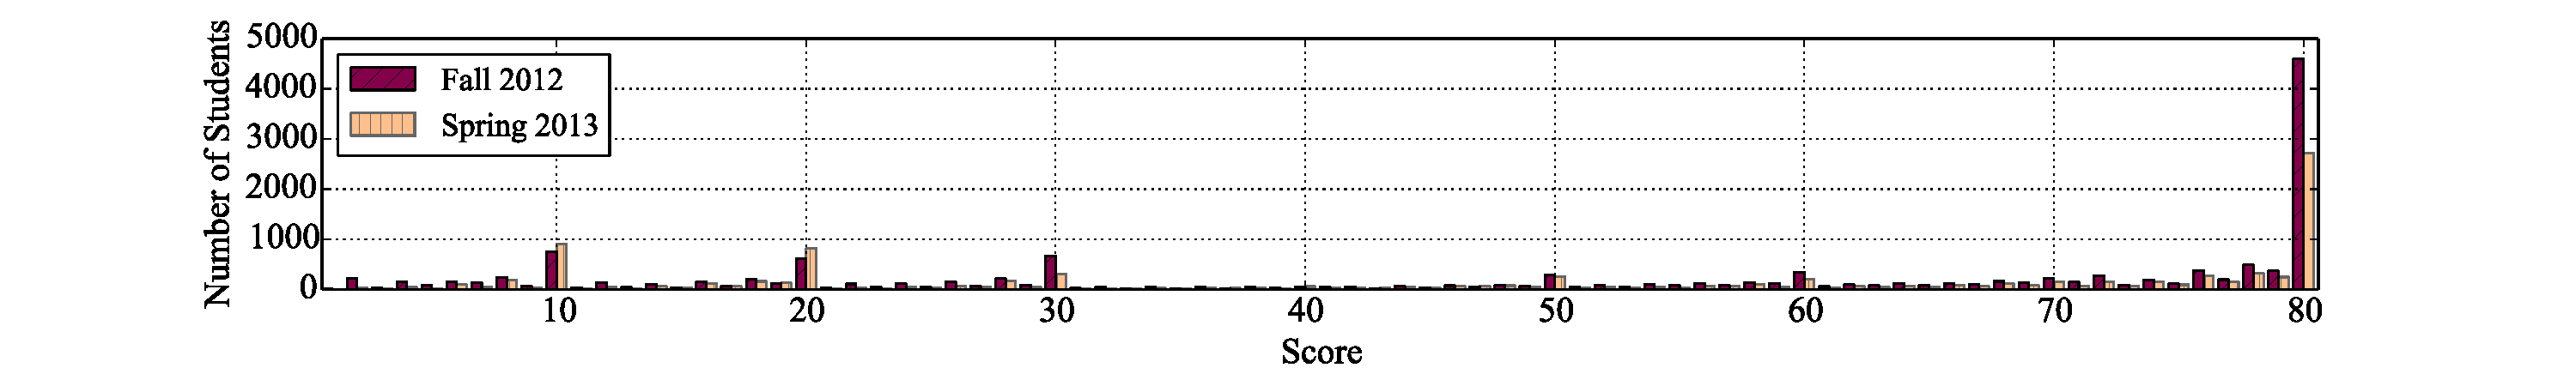
\includegraphics[width=\textwidth]{plots/final-scores.pdf}
  \caption{Final scores after the entire course (both iterations).}
  \label{fig:final-scores}
\end{figure*}

\subsection{Assignments, submissions, and grades}

In this section we evaluate statistics obtained through the MOOC platform such
as final grades, per-assignment grades, and the number of re-submissions per
assignment. In the process, we present several correlations between
submissions and grades. Furthermore, we compare statistics obtained for two
different iterations of the MOOC. The results can provide insight into the
usage of the assignment submission system, and how it affects students'
grades.


\begin{figure*}[ht!]
  \centering
  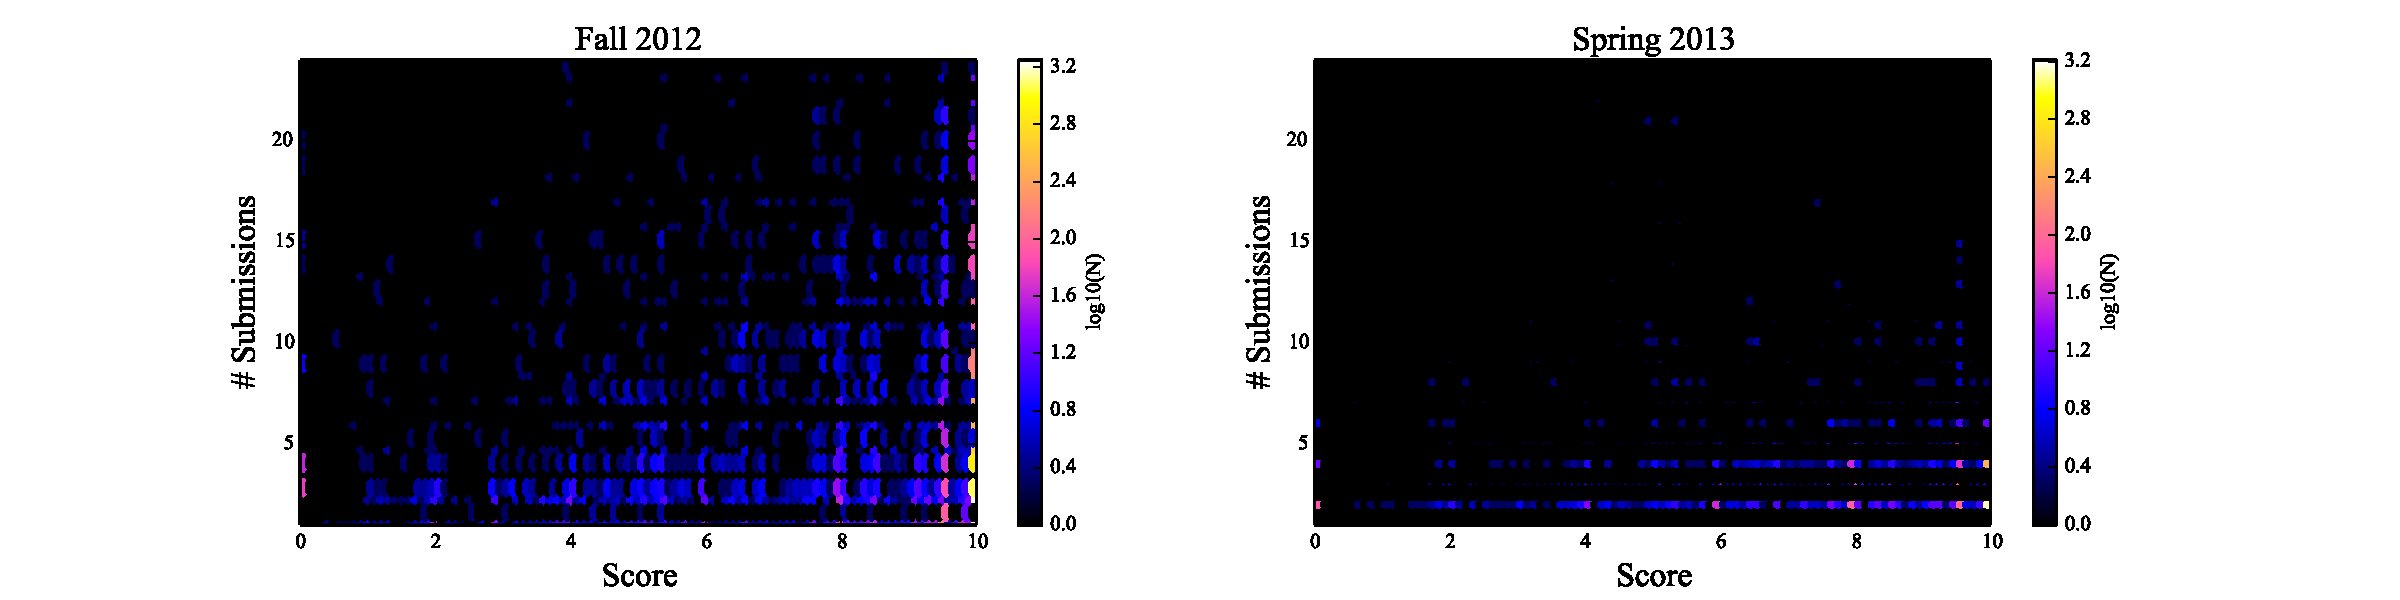
\includegraphics[width=\textwidth]{plots/score-2d-histogram-fall2012-spring2013.pdf}
  \caption{Heat maps correlating scores for the ``Huffman'' assignment and the number
  of required submissions.}
  \label{fig:2d-histogram}
\end{figure*}

\subsubsection{Grading policies}\label{sec:grading-policies}

As mentioned in Section~\ref{sec:mooc-elements} the grading policy changed
between the Fall 2012 and the Spring 2013 iterations of the course. In the
Fall 2012 iteration, students could re-submit solutions as often as they
wanted without penalty until the submission deadline. In the Spring 2013
iteration, students were allowed to re-submit only up to five times; the sixth
and later submissions would not give any credit. In both iterations the
(valid) submission with the highest grade determined the final grade for that
assignment.

\subsubsection{Correlating grade and number of submissions}

Figure~\ref{fig:2d-histogram} shows the correlation between the achieved
score for one particular assignment (an implementation of Huffman coding using
pattern matching) and the number of submissions required of each student to achieve that
score. For both the Fall 2012 and the Spring 2013 iterations of the course,
the largest concentration of students at or close to the perfect score
(10). In fact, a large number of students required only five submissions or less to
achieve their final/best score. Moreover, the results suggest that to achieve
a higher score, a higher number of submissions was {\em not usually necessary}.

However, for the Fall 2012 iteration there are still thousands of students
with 10 or even 15 submissions. The results for the Spring 2013 iteration are
quite different: most people achieved their final score after only two or four
submissions. This is very likely due to the different grading policies used in
the two iterations: the grading policy in Spring 2013 does not give credit for
the sixth and later submissions. This is clearly reflected in the changed
submission statistics. However, interestingly there is still a significant
number of students who also submitted a sixth time (thus earning no additional
credit); this is a clear indication that the automated grading and feedback
was also used for learning without improving one's score.

\begin{figure}[ht!]
  \centering
  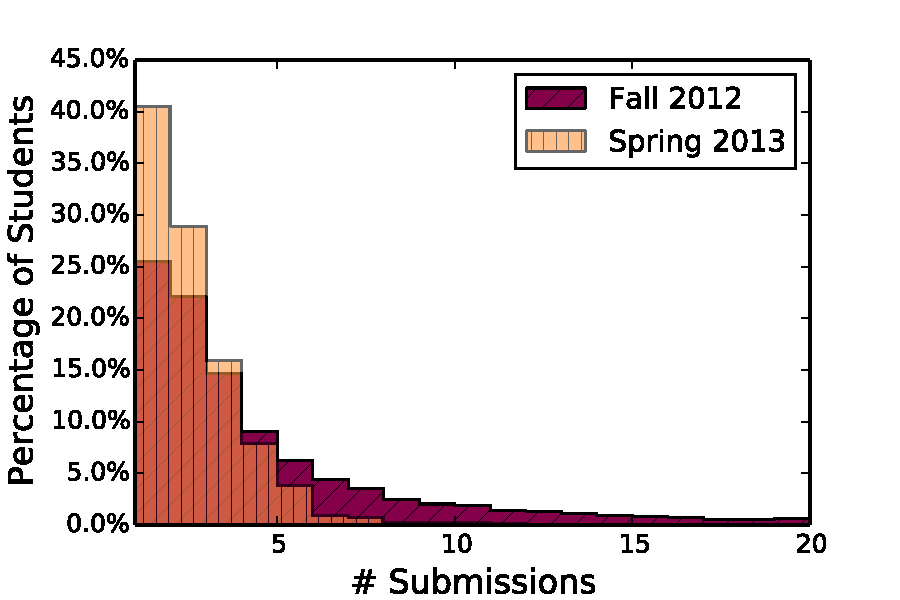
\includegraphics[width=\columnwidth]{plots/top-scores-submissions-histogram.pdf}
  \caption{The number of submissions required to achieve a perfect score in the ``Huffman'' assignment.}
  \label{fig:top-scores-submissions}
\end{figure}

\begin{figure*}[ht!]
  \centering
  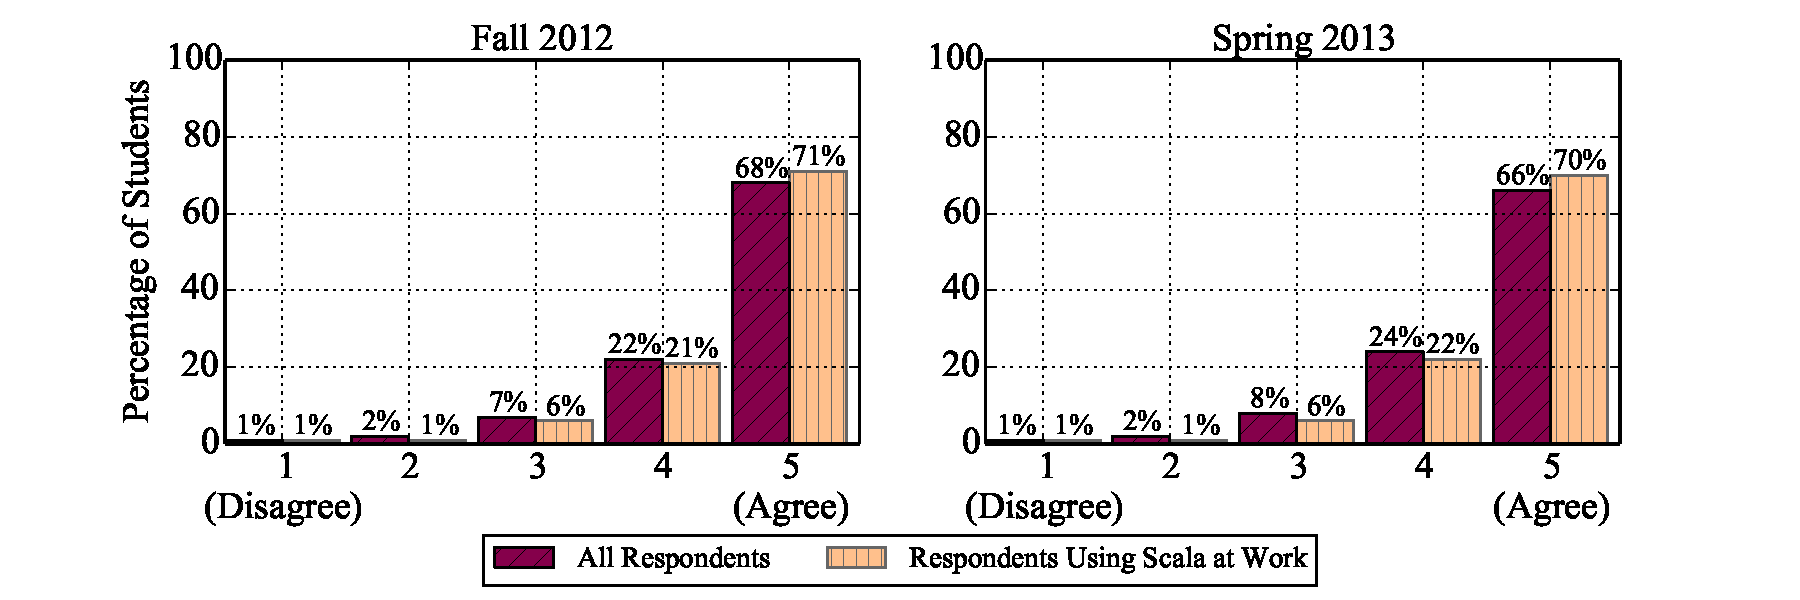
\includegraphics[width=\textwidth]{plots/worth-it-apply-it.pdf}
  \caption{}
  \label{fig:worth-it-apply-it}
\end{figure*}

\begin{figure*}[ht!]
  \centering
  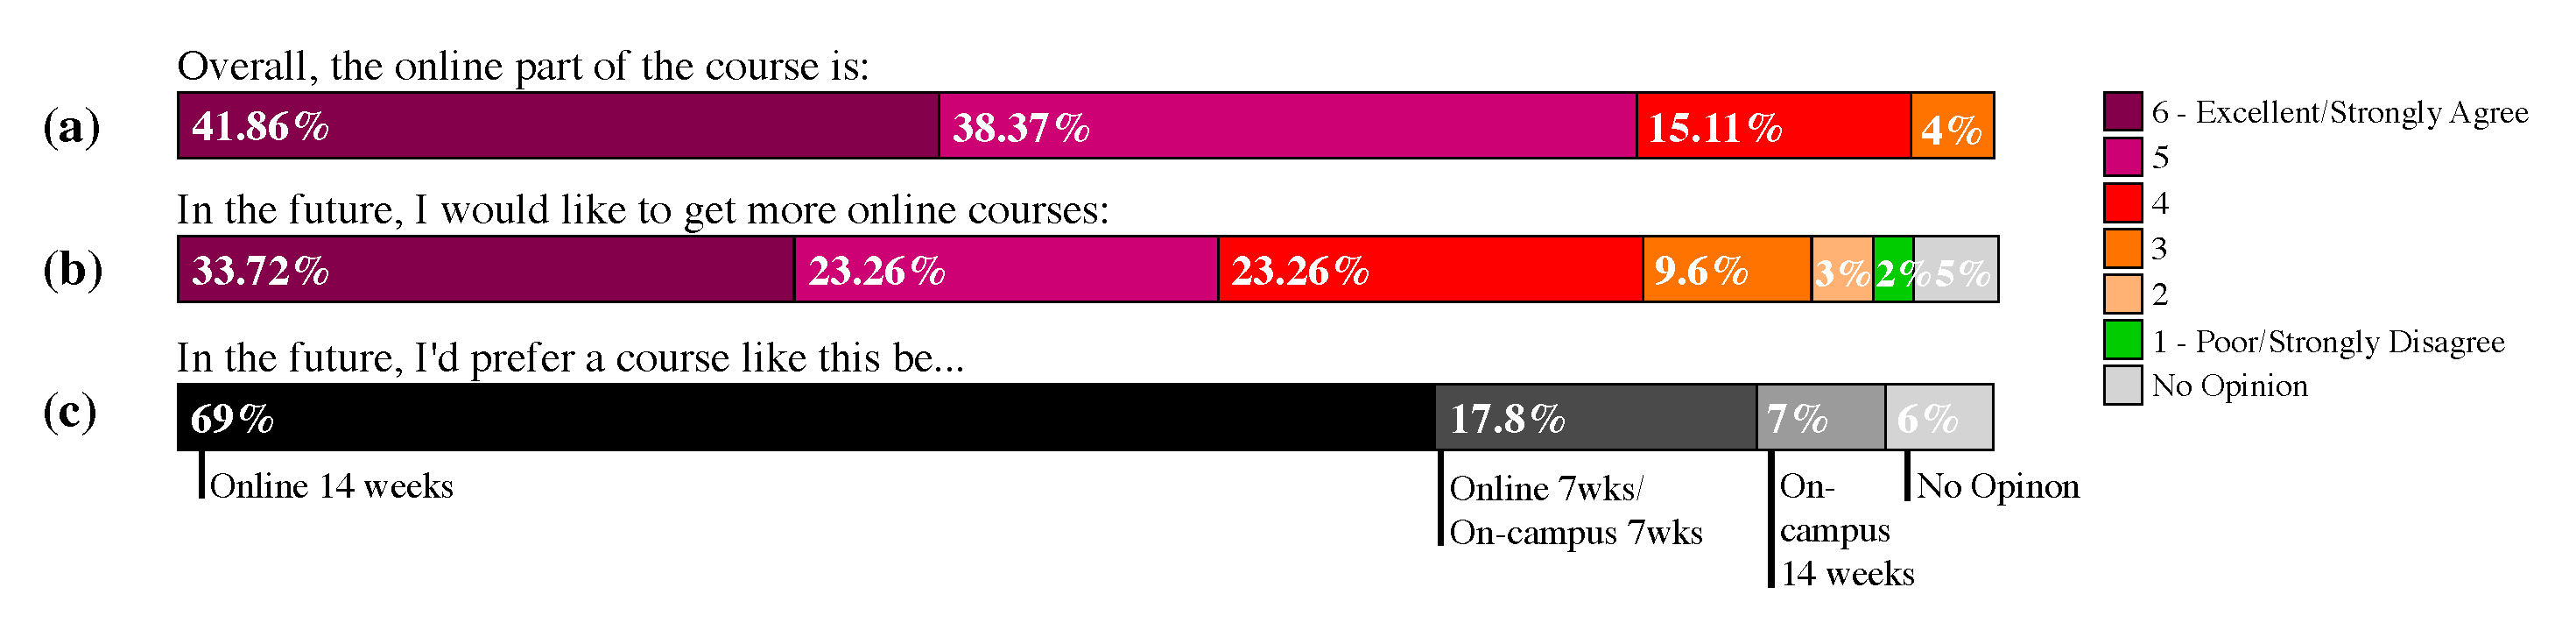
\includegraphics[width=\textwidth]{plots/epfl-course-eval.pdf}
  \caption{}
  \label{fig:epfl-course-eval}
\end{figure*}


\subsubsection{Evaluating the grading policy}\label{sec:eval-grading-policy}

This change in the grading policy had an interesting effect on the number of
submitted solutions. Figure~\ref{fig:top-scores-submissions} shows the change
in the number of submissions of students who achieved a perfect score on a
particular assignment. The change in submission behavior is quite noticeable.
In the Fall 2012 iteration about 25\% of those perfect-scorers needed only one
submission, whereas in the Spring 2013 iteration this percentage grew to about
40\%. For perfect-scorers who needed two submissions, the difference between
the two iterations is not as large, but still significant (an increase of
about 30\%).

\subsection{Post-course survey results}


\subsection{Explaining the high completion rate}

Show how people used the submission system. People were ``hooked'' on submitting solutions.

\begin{itemize}

\item what we can show is how people used the submission system (how often submitted, how
  many points on final submission)

\item we can also show how many people submitted solutions until the end (did the points
  earned by submitting go down or not? If so, by how much?)

\item so, if we can somehow show that people got ``hooked'' on submitting solutions, then
  the setup of allowing multiple (unbounded) submissions with immediate feedback was
  successful: submitting was motivating

\end{itemize}

Examine motivation and background of participants. A lot of the motivation for
people completing the course could come from the fact that they were trying to
learn something that's important for the job, and something that they can't
get anywhere else in a comparable form (indeed, Scala is not yet taught in
many universities). Survey results indicate that about 40\% of respondents
plan to apply the learned knowledge at work. Of those 40\% respondents, we
found that ??\% said that the course was well worth their time (thus, it was
``effective'' for learning). [New correlation] These results also indicate
that MOOCs are an effective training tool for practicing software engineers.

Furthermore, a certificate of completion was issued. Unlike languages
established in industry for many years, there is no standard Scala
certification for developers; the completion certificate could be regarded by
many as the closest substitute.

\subsection{The role of new tools for teaching and learning}

[submission system]

Furthermore, survey results show (see Figure~\ref{fig:ide-usage}) that the use
of the new worksheet technology lead to a doubling in the percentage of use of
the Eclipse IDE compared to a non-course setting. Thus, the worksheet was a
very strong incentive for people to use Eclipse during the course. Again, the
worksheet fundamentally changed the way people interacted with the course
material. The use of Eclipse was voluntary; in fact, many people used other
IDEs such as IntelliJ IDEA. However, even so, the use of Eclipse was so much
higher than usual. Thus, people welcomed the difference in learning that the
worksheet enabled.

\subsection{Educational Background}

[It turns out most participants already have a degree.]

[We also have results for the question: why did you chose to do the course.]

\subsection{Course Completion Rate}

At the time the first iteration of the progfun course was completed, the
course had one of the highest completion rate of any MOOC world-wide [needs
citation: http://www.katyjordan.com/MOOCproject.html].

Could be good to cite, too:~\cite{Parr13}

\section{Related Work}


For example, the well-known MOOC on software engineering organized by Fox and
Patterson~\cite{FoxP12} has had around 50'000 registered students in its first
iteration, and is thus comparable in size to our course; however, no survey of
a comparable size was conducted among participants of the MOOC. Moreover, our
selection of questions provides new insights, related to the interplay of
MOOCs with professional software engineering, in particular.


Vihavainen et al. report on a MOOC ("Helsinki MOOC") on introductory computer
science with an emphasis on programming~\cite{VihavainenLK12}. Compared to the
Helsinki MOOC, our course had a number of registered students two orders of
magnitude larger. Moreover, the Helsinki MOOC targets introductory
programming, whereas our course targets advanced programming principles. As a
result, our course was very popular especially among advanced developers who
already have a Bachelor's or Master's degree. The Helsinki MOOC does not treat
university students and MOOC participants equal with respect to the material
used for exercises: the students in their university course are beta testers
of the exercise material; thus, only after this beta test and necessary
adjustments is the material released to non-local MOOC participants. Other
organizational differences exist. For example, they give formal credits for
``apprentices'' who are unpaid ``advisors'' among fellow students with limited
responsibilities. Their Extreme Apprenticeship (XA) learning methodology
required a staff of around 20 persons associated with the course, with
different roles and responsibilities. It is unclear whether the XA methodology
would scale to a course of the scale of progfun (50'000 registered students
versus 500 registered students).


%
% The following two commands are all you need in the
% initial runs of your .tex file to
% produce the bibliography for the citations in your paper.
\bibliographystyle{abbrv}
\bibliography{sigproc}  % sigproc.bib is the name of the Bibliography in this case
% You must have a proper ".bib" file
%  and remember to run:
% latex bibtex latex latex
% to resolve all references
%
% ACM needs 'a single self-contained file'!
%
%APPENDICES are optional
%\balancecolumns
\end{document}
